\documentclass{../../submodules/TEX/document/ug/ug}
\usepackage{float}
\usepackage{color, colortbl}
\usepackage[section]{placeins}
\usepackage{mathtools}
\usepackage{amsthm}
%\usepackage[T1]{helvet}
\usepackage[OT1]{fontenc} 


\theoremstyle{plain}
\newtheorem*{defn*}{Definition}
\newtheorem*{ex*}{Example}


\title{IObundle IOb SPI Flash Controller User Guide}
\category{User Guide}

%\getenv[\TEX]{TEX_DIR}
\input{\TEX/color}

\begin{document}
\maketitle
\cleardoublepage
\tableofcontents
\clearpage
\listoftables
\clearpage
\listoffigures
\cleardoublepage

\section{\textcolor[rgb]{0,0,0}{Introduction}}
The IObundle xSPI Flash Controller core is a configurable spi/xspi master interface core
for communication with flash memories. It supports automatic controller configuration,
Execute-in-Place (XiP) mode, simple and multi-line dual/quad communication protocols
and STR (Single Transfer Rates)/DDR (Double Data Rates) modes. 
The IP is currently supported for use in ASICs and FPGAs.


\section{Symbol}
\begin{figure}[!htbp]
    \centerline{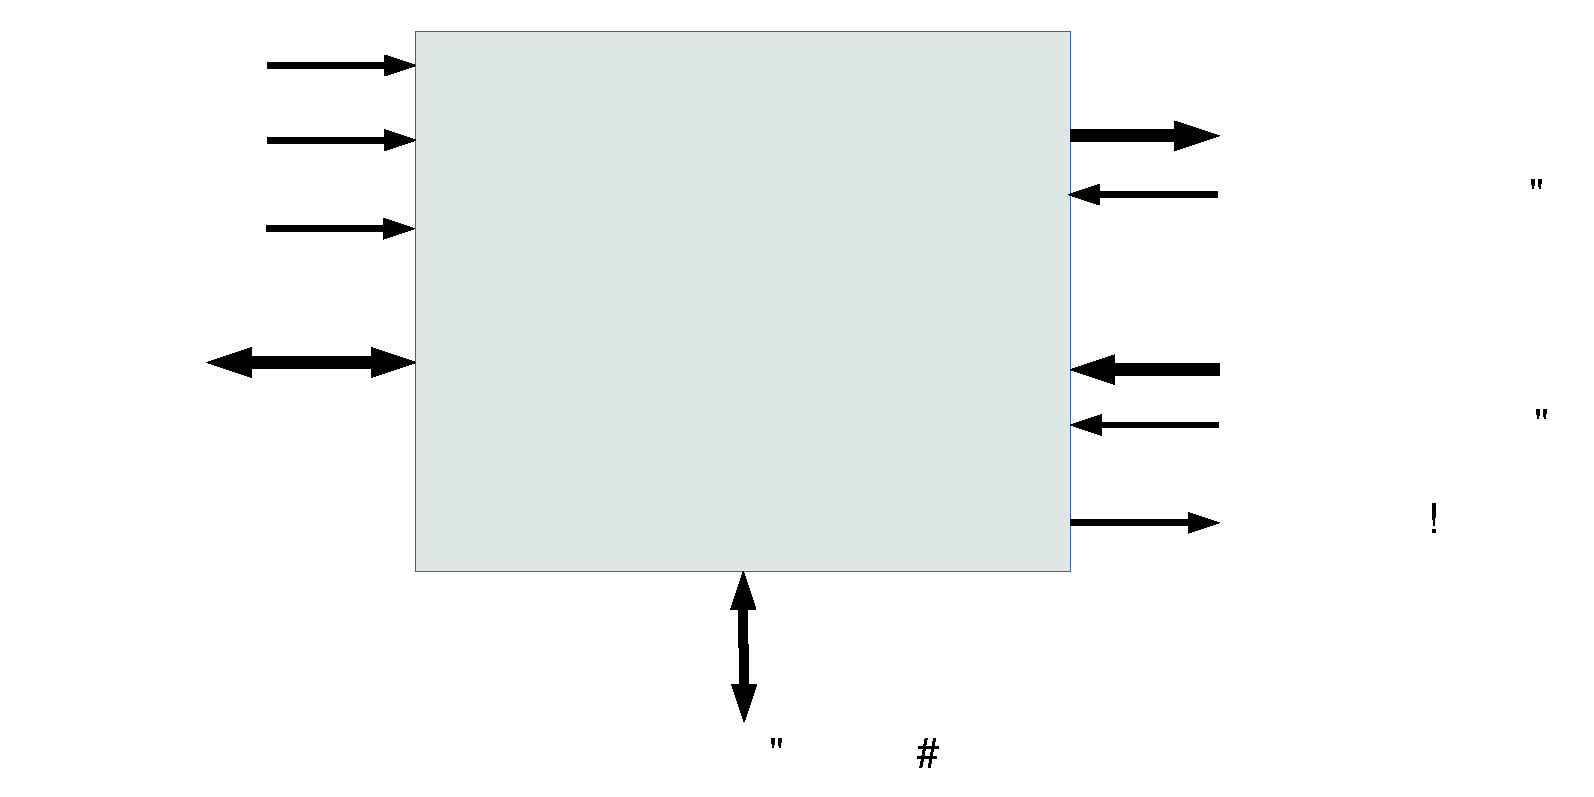
\includegraphics[width=14cm]{symb.pdf}}
    \vspace{0cm}\caption{IP Core Symbol}
    \label{fig:i2score_sym}
\end{figure}



\section{\textcolor[rgb]{0,0,0}{Features}}
 \begin{itemize}
	\item Iob Native interface support
	\item Configurable spi data lanes: 1, 2 (dual) or 4 (quad) lane modes
	\item Supports eXecute-In-Place (XIP) mode for low latency
		memory reads, requiring only memory address. Allows for code execution
		directly on flash
		access
	\item Supports STR (Single Data Rate) and DTR (Double Data Rate) for increased
		throughput in low frequency systems
	\item Flexible configurable frame format
 \end{itemize}


\section{\textcolor[rgb]{0,0,0}{Benefits}}
\begin{itemize}
\item Easy hardware and software integration
\item Compact hardware implementation
\item Can fit many instances in low cost FPGAs
\item Can fit many instances in small ASICs 
\item Low power consumption
\end{itemize}


\section{\textcolor[rgb]{0,0,0}{Deliverables}}
\begin{itemize}
	\item ASIC or FPGA synthesized netlist or Verilog source code
	\item Software driver and example user software
	\item User documentation for easy system integration
	\item Example integration in IOb-SoC (optional)
\end{itemize}


\section*{\textcolor[rgb]{0,0,0}{Block Diagram}}
\begin{figure}[H]
  \vspace{-.5cm}
  \centering {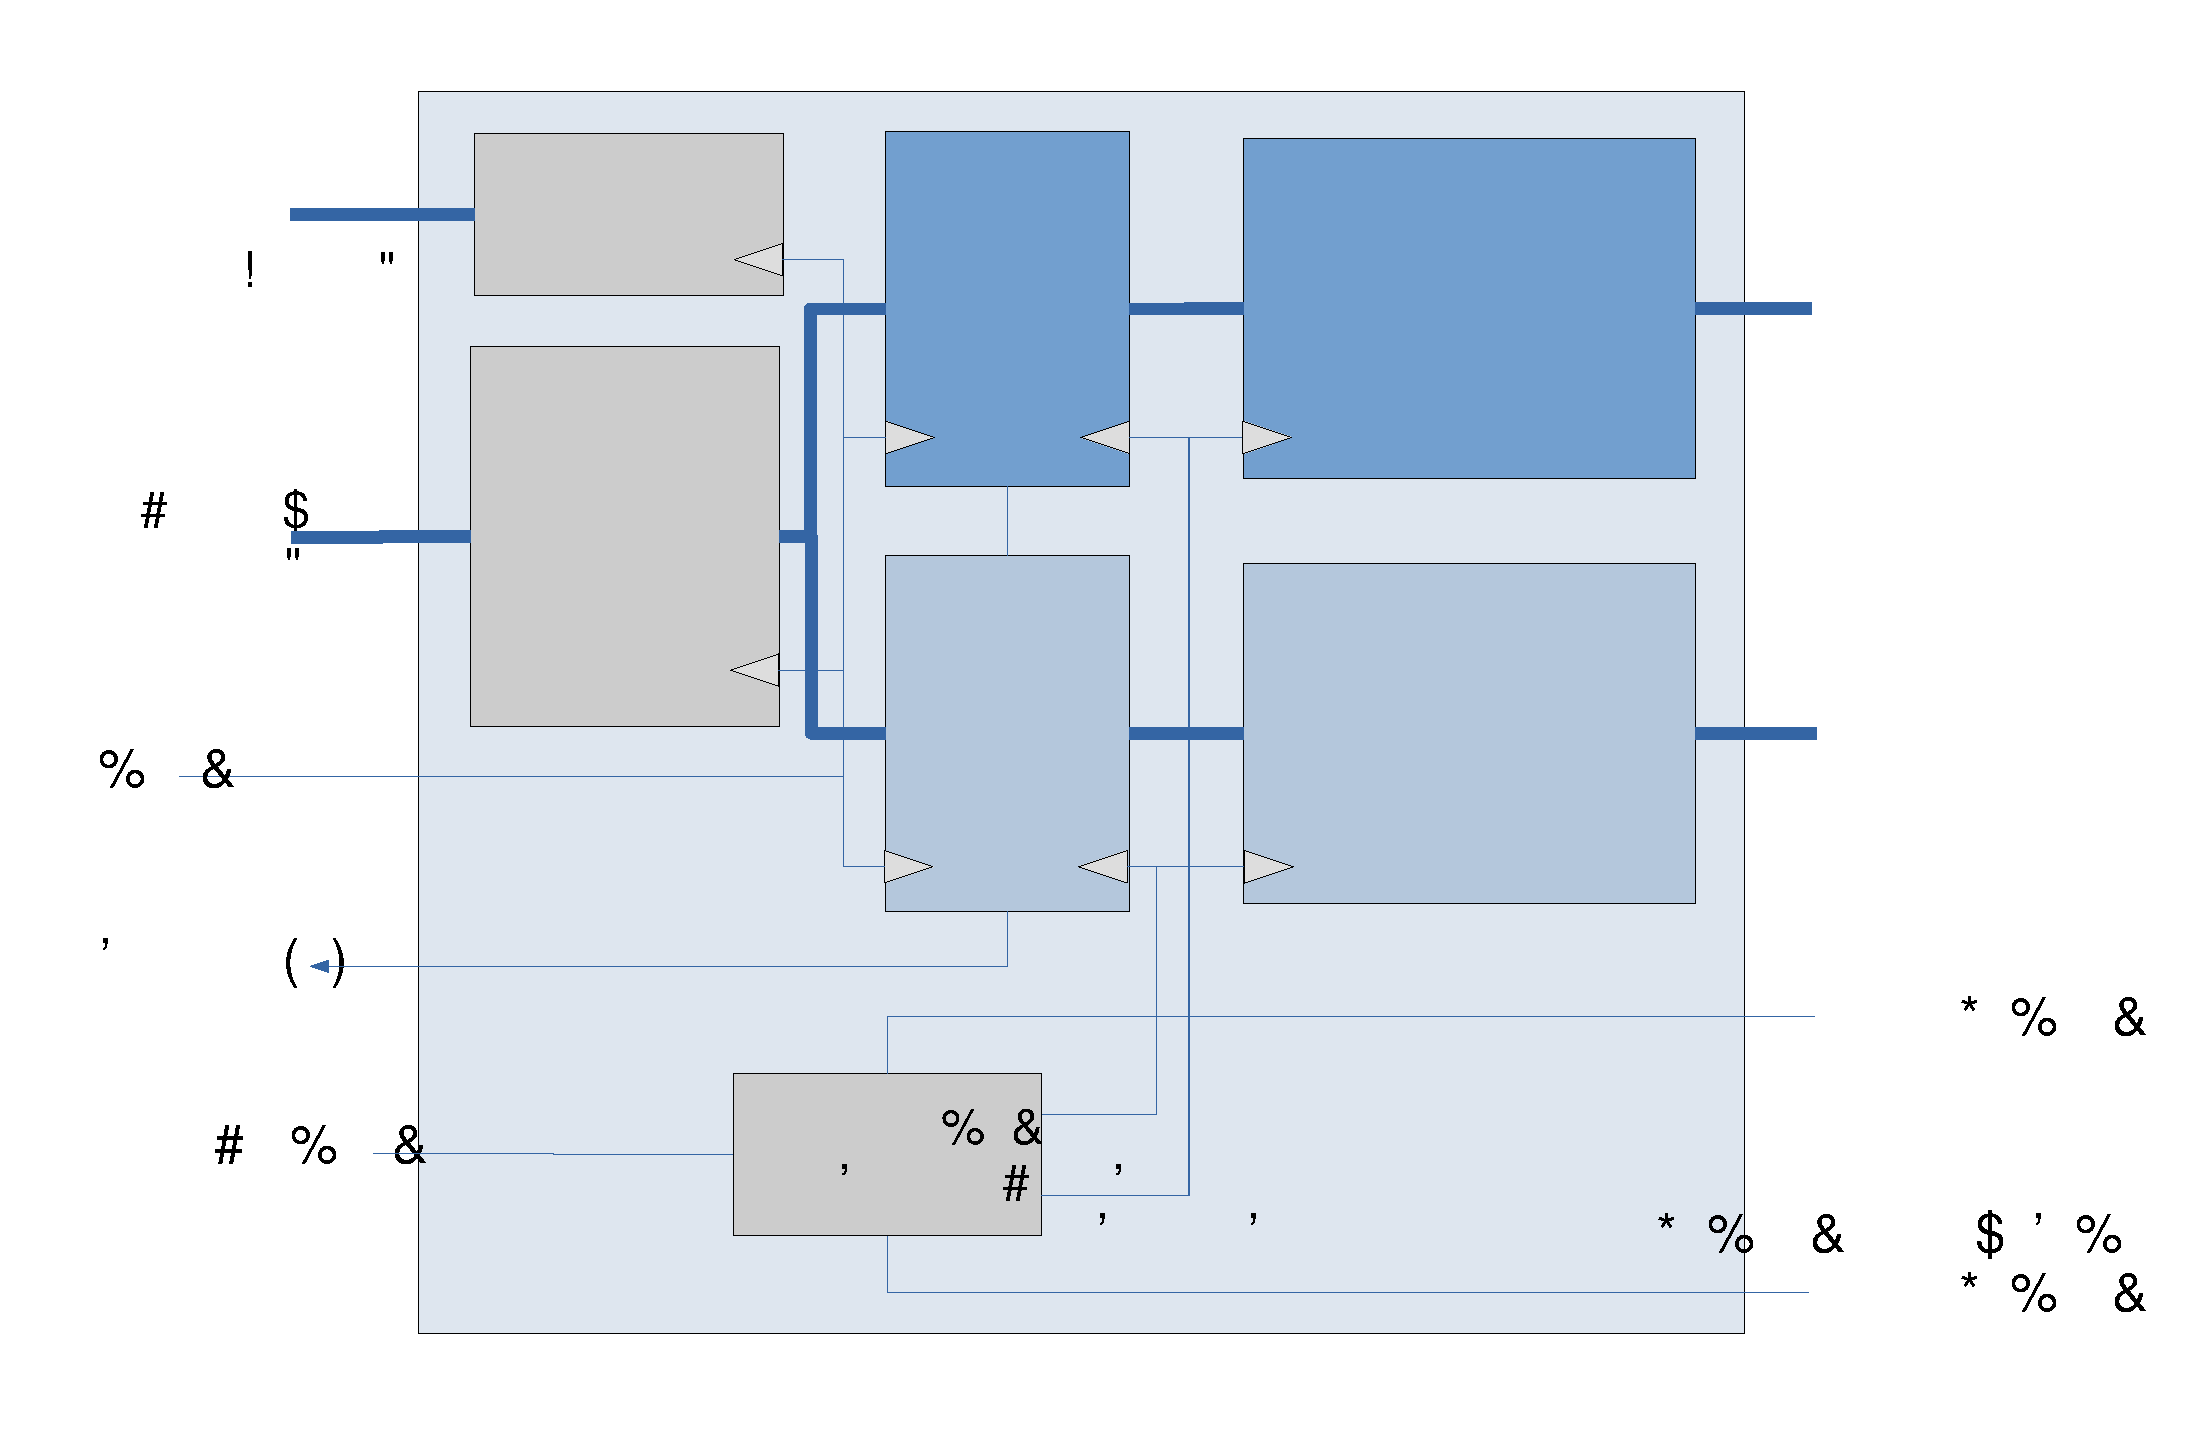
\includegraphics[width=\columnwidth]{bd.pdf}}
  \label{fig:bd}
  \vspace{-0.7cm}
  \caption{High-level block diagram}
\end{figure}


\section{Interface Signals}

\begin{table}[t]
  \begin{center}
    \begin{tabular}{|l|l|p{8cm}|}
      \hline
      \rowcolor{iob-green}
      \textbf{Signal} & \textbf{Direction} & \textbf{Description} \\
      clk & Input & system clock signal\\
      rst & Input & system reset signal\\
      valid & Input & 1-bit\\
      address & Input & 4-bit select SW Register\\
      wdata & Input & 32-bit data to write to SW Register\\
      wstrb & Input & 4-bit byte to write\\
      rdata & Output & 32-bit data to read\\
      ready & Output & 1-bit idle state\\
      valid\_cache & Input & 1-bit instructions i/f\\
      address\_cache & Input & 24-bit instructions i/f flash address\\
      wdata\_cache & Input & 32-bit instructions i/f UNUSED\\
      wstrb\_cache & Input & 4-bit intructions i/f byte to write\\
      rdata\_cache & Output & 2-bit intructions i/f data read\\
      ready\_cache & Output & 1-bit instructions i/f\\
      SS & Output & SPI i/f \\
      SCLK & Output & SPI i/f serial clock\\
      MOSI & Bidir & SPI i/f DQ0\\
      MISO & Bidir & SPI i/f DQ1\\
      WP\_N & Bidir & SPI i/f DQ2\\
      HOLD\_N & Bidir & SPI i/f DQ3\\
      \hline
      \hline

     % \input is_tab.tex

    \end{tabular}
    \caption{General interface signals}
    \label{tab:is}
  \end{center}
\end{table}


\section{Timing Diagrams}

\begin{figure}[H]
  \begin{center}
    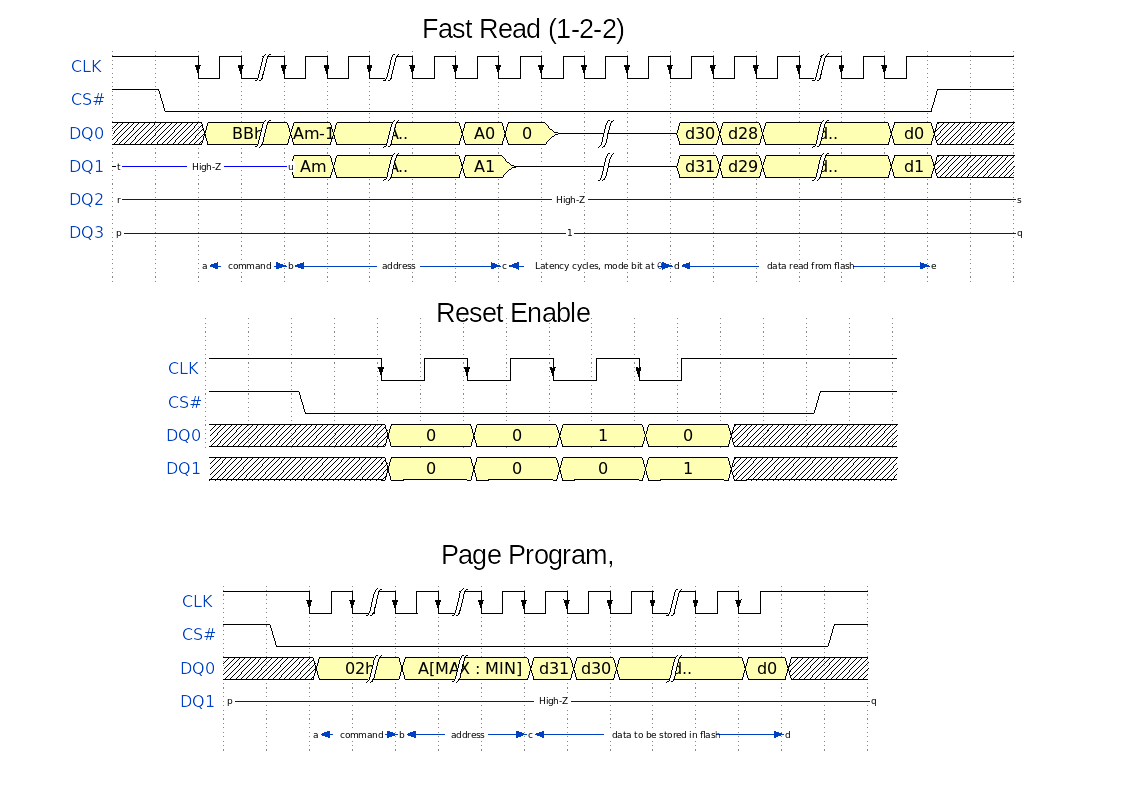
\includegraphics[width=16cm]{spi.png}
    \caption{SPI slave interface timing diagram}
    \label{fig:spi}
  \end{center}
\end{figure}

\section{Software Components}
A set of SW accessible Registers interacting basic functions (platform functions) are provided.
Higher level functions can be built on top of the platform functions, with several already provided
which implement support for select flash commands.

\section*{FPGA Resources}
The following are FPGA implementation results for two FPGA device families. 

The following are FPGA implementation results for two FPGA device families. 

The following are FPGA implementation results for two FPGA device families. 

\input{\TEX/fpga}





%\bibliographystyle{unsrt}
%\bibliography{rep}
%\nocite{*}

\end{document}
